\documentclass[12pt,a4paper]{article}
\usepackage[utf8]{vietnam}
\usepackage{amsmath}
\usepackage{amsfonts}
\usepackage{xcolor}
\usepackage{titlesec}
\usepackage{mdframed}
\usepackage{amssymb}
\usepackage{pgf,tikz,pgfplots}
\usepackage{graphicx}
\usepackage{cases} 
\pgfplotsset{compat=1.5}
\usepackage{mathrsfs}
\usetikzlibrary{arrows, calc}
\usepackage{fancyhdr}
\pagestyle{fancy}
\pagestyle{empty}
\usepackage[left=2cm,right=2cm,top=2cm,bottom=2cm]{geometry}
\author{Nguyễn Văn Lộc}
\newmdenv[linecolor=black,skipabove=\topsep,skipbelow=\topsep,
leftmargin=-5pt,rightmargin=-5pt,
innerleftmargin=5pt,innerrightmargin=5pt]{mybox}
\begin{document}
\fancyhf{}
\lhead{}
\chead{}
\rhead{}
\cfoot{\thepage}
\rfoot{}
\lfoot{}
\pagestyle{fancy}
\renewcommand{\headrulewidth}{0pt}
\renewcommand{\footrulewidth}{0pt}
\begin{flushleft}
	\begin{mybox}
	\textbf{Họ và tên:} Nguyễn Văn Lộc\\
	\textbf{MSSV:} 20120131\\ 
	\textbf{Lớp:} 20CTT1TN\\
	\textbf{Ca:} Ca 1 sáng thứ 4
	\end{mybox}
\end{flushleft}
\begin{center}
	\textbf{BÀI TẬP THỰC HÀNH VI TÍCH PHÂN 2B}\\
	\textbf{CHƯƠNG 4: GIẢI TÍCH VECTOR}
\end{center}
\textbf{Trang 74.}\\
\textbf{Bài 3.}
\begin{mybox}
	Tính tích phân đường \(I = \int_C {x{y^4}} ds\) với \(C\) là nửa bên 	phải của đường tròn \({x^2} + {y^2} = 16.\)
\end{mybox}
\begin{center}
	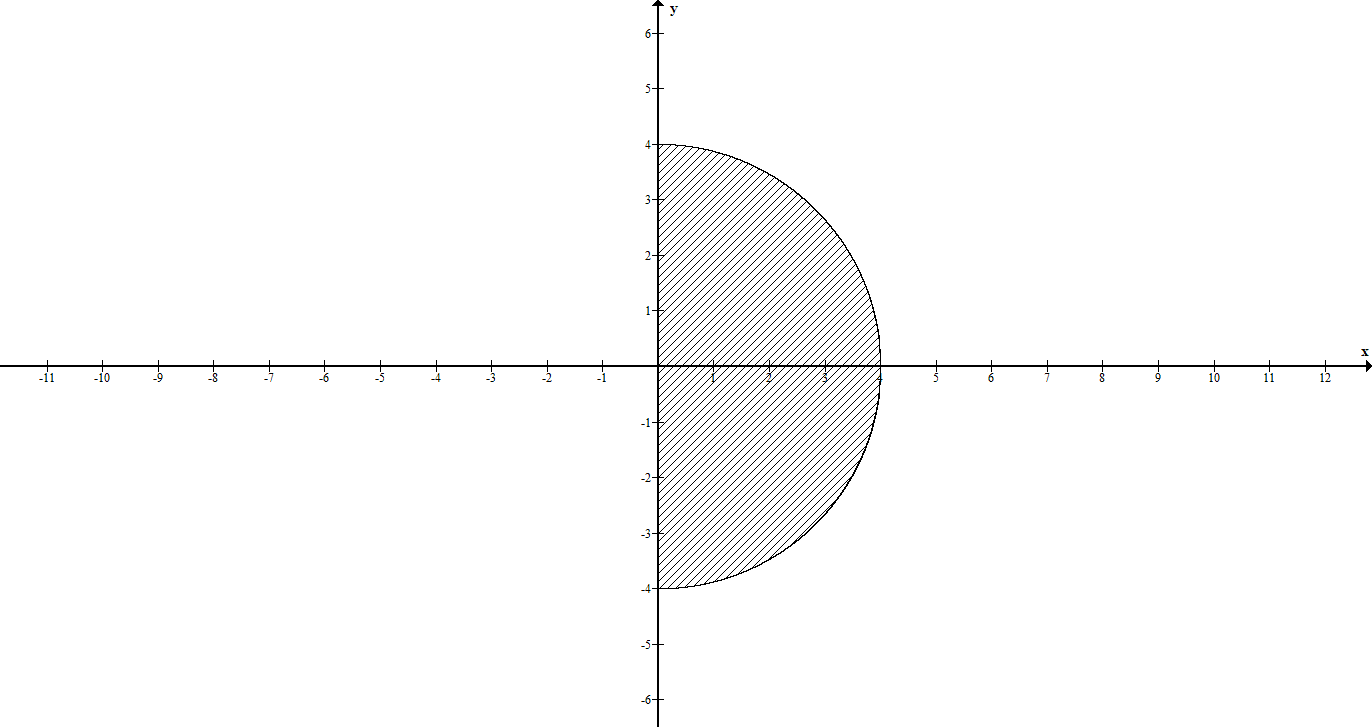
\includegraphics[scale=0.3]{c4_1}
\end{center}
Một tham số của đường cong \(C\) là
\[\left\{ \begin{gathered}
  x = 4\cos t \hfill \\
  y = 4\sin t \hfill \\ 
\end{gathered}  \right.,t \in \left[ { - \frac{\pi }{2},\frac{\pi }{2}} \right].\]
\[ \Rightarrow \left\{ \begin{gathered}
  \frac{{dx}}{{dt}} =  - 4\sin t \hfill \\
  \frac{{dy}}{{dt}} = 4\cos t \hfill \\ 
\end{gathered}  \right..\]
\[ \Rightarrow I = \int\limits_{ - \frac{\pi }{2}}^{\frac{\pi }{2}} {4\cos t \cdot {{\left( {4\sin t} \right)}^4}\sqrt {{{\left( { - 4\sin t} \right)}^2} + {{\left( {4\cos t} \right)}^2}} dt} \]
\[ \Rightarrow I = 4096\int\limits_{ - \frac{\pi }{2}}^{\frac{\pi }{2}} {{{\sin }^4}t\cos tdt = \left. {4096 \cdot \frac{{{{\sin }^5}t}}{5}} \right|} _{t =  - \frac{\pi }{2}}^{t = \frac{\pi }{2}} = \frac{{8192}}{5}.\]
\textbf{Bài 4.}
\begin{mybox}
	Tính tích phân đường \(I = \int_C {x\sin yds} \) với \(C\) là đoạn 	
	thẳng nối từ \(\left( {0,3} \right)\) đến \(\left( {4,6} \right).\)
\end{mybox}
\begin{center}
	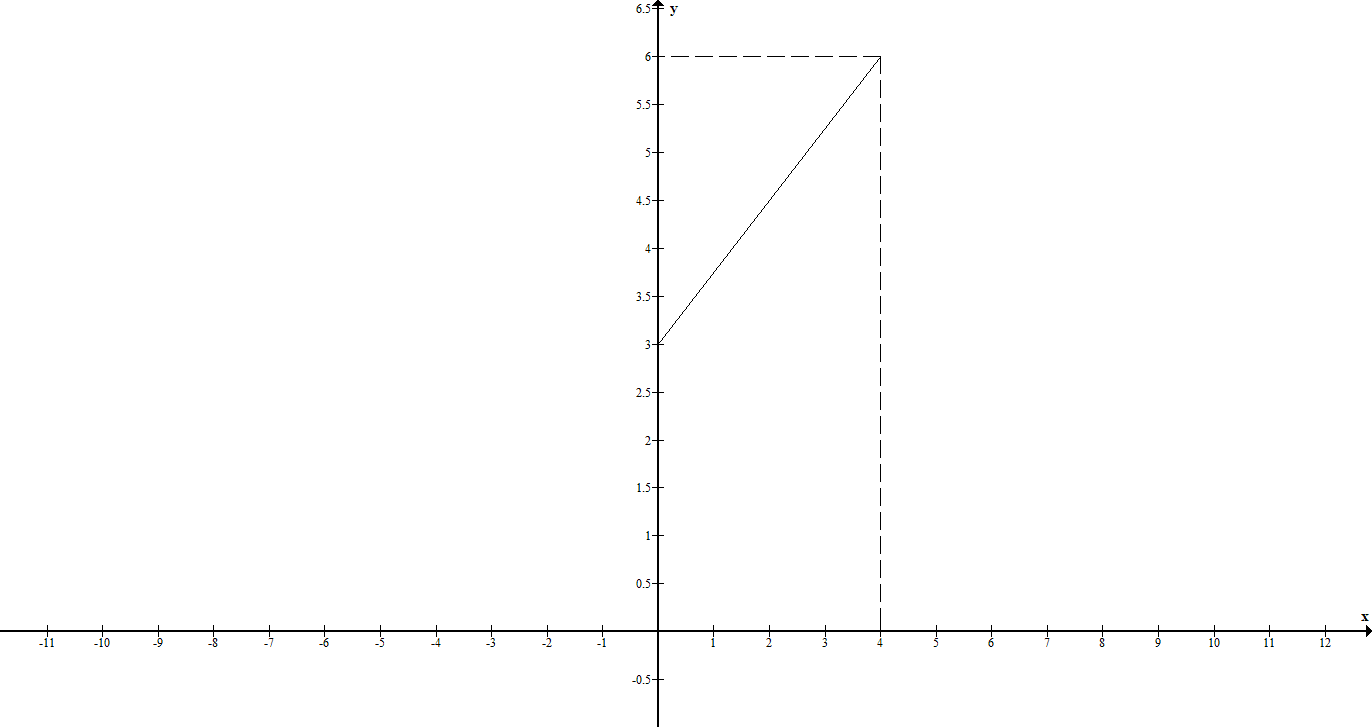
\includegraphics[scale=0.3]{c4_2}
\end{center}
Phương trình đường thẳng nối từ \(\left( {0,3} \right)\) đến \(\left( {4,6} \right)\) là \(y = \frac{3}{4}x + 3.\)\\
Một tham số của \(C\) là
\[\left\{ \begin{gathered}
  x = t \hfill \\
  y = \frac{3}{4}t + 3 \hfill \\ 
\end{gathered}  \right.,t \in \left[ {0,4} \right].\]
\[ \Rightarrow \left\{ \begin{gathered}
  \frac{{dx}}{{dt}} = 1 \hfill \\
  \frac{{dy}}{{dt}} = \frac{3}{4} \hfill \\ 
\end{gathered}  \right..\]
\[ \Rightarrow I = \int\limits_0^4 {t\sin \left( {\frac{3}{4}t + 3} \right)\sqrt {{1^2} + {{\left( {\frac{3}{4}} \right)}^2}} dt} \]
\[ \Rightarrow I = \frac{5}{4}\int\limits_0^4 {t\sin \left( {\frac{3}{4}t + 3} \right)dt}. \]
Đặt \(\left\{ \begin{gathered}
  u = t \hfill \\
  dv = \sin \left( {\frac{3}{4}t + 3} \right)dt \hfill \\ 
\end{gathered}  \right. \Rightarrow \left\{ \begin{gathered}
  du = dt \hfill \\
  v =  - \frac{4}{3}\cos \left( {\frac{3}{4}t + 3} \right) \hfill \\ 
\end{gathered}  \right..\)
\[ \Rightarrow I = \frac{5}{4}\left[ {\left. { - \frac{4}{3}t\cos \left( {\frac{3}{4}t + 3} \right)} \right|_{t = 0}^{t = 4} + \frac{4}{3}\int\limits_0^4 {\cos \left( {\frac{3}{4}t + 3} \right)dt} } \right]\]
\[ \Rightarrow I = \frac{5}{4}\left[ { - \frac{4}{3}\left( {\cos 6 - \cos 3} \right) + \frac{4}{3} \cdot \frac{4}{3}\left. {\sin \left( {\frac{3}{4}t + 3} \right)} \right|_{t = 0}^{t = 4}} \right]\]
\[ \Rightarrow I = \frac{5}{4}\left[ { - \frac{4}{3}\left( {\cos 6 - \cos 3} \right) + \frac{{16}}{9}\left( {\sin 6 - \sin 3} \right)} \right]\]
\[ \Rightarrow I =  - \frac{5}{3}\left( {\cos 6 - \cos 3} \right) + \frac{{20}}{9}\left( {\sin 6 - \sin 3} \right).\]
\textbf{Bài 5.}
\begin{mybox}
Tính tích phân đường \(I = \int_C {xyzds} \) với \(C:x = 2\sin t,y = t,z =  - 2\cos t,0 \leqslant t \leqslant \pi. \)
\end{mybox}
Một tham số của \(C\) là 
\[C:\left\{ \begin{gathered}
  x = 2\sin t \hfill \\
  y = t \hfill \\
  z =  - 2\cos t \hfill \\ 
\end{gathered}  \right.,t \in \left[ {0,\pi } \right].\]
\[ \Rightarrow \left\{ \begin{gathered}
  \frac{{dx}}{{dt}} = 2\cos t \hfill \\
  \frac{{dy}}{{dt}} = 1 \hfill \\
  \frac{{dz}}{{dt}} = 2\sin t \hfill \\ 
\end{gathered}  \right..\]
\[ \Rightarrow I = \int\limits_0^\pi  {2\sin t \cdot t \cdot } \left( { - 2\cos t} \right)\sqrt {{{\left( {2\cos t} \right)}^2} + {1^2} + {{\left( {2\sin t} \right)}^2}} dt\]
\[ \Rightarrow I =  - 2\sqrt 5 \int\limits_0^\pi  {t\sin \left( {2t} \right)} dt = \sqrt 5 \int\limits_0^\pi  {t \cdot \left( { - 2\sin \left( {2t} \right)} \right)} dt.\]
Đặt \(\left\{ \begin{gathered}
  u = t \hfill \\
  dv =  - 2\sin \left( {2t} \right)dt \hfill \\ 
\end{gathered}  \right. \Rightarrow \left\{ \begin{gathered}
  du = dt \hfill \\
  v = \cos \left( {2t} \right) \hfill \\ 
\end{gathered}  \right..\)
\[ \Rightarrow I = \sqrt 5 \left[ {\left. {t\cos \left( {2t} \right)} \right|_{t = 0}^{t = \pi } - \int\limits_0^\pi  {\cos \left( {2t} \right)dt} } \right]\]
\[ \Rightarrow I = \sqrt 5 \left[ {\pi  - \left. {\frac{1}{2}\sin \left( {2t} \right)} \right|_{t = 0}^{t = \pi }} \right] = \pi \sqrt 5 .\]
\textbf{Trang 77.}\\
\textbf{Bài 1.}
\begin{mybox}
Tính tích phân đường loại \(2:\) \(I = \int_C {\left( {{x^2}{y^3} - \sqrt x } \right)}dy \) với \(C\) là đoạn cong \(y = \sqrt x \) từ \(\left( {1,1} \right)\) đến \(\left( {4,2} \right).\)
\end{mybox}
\begin{center}
	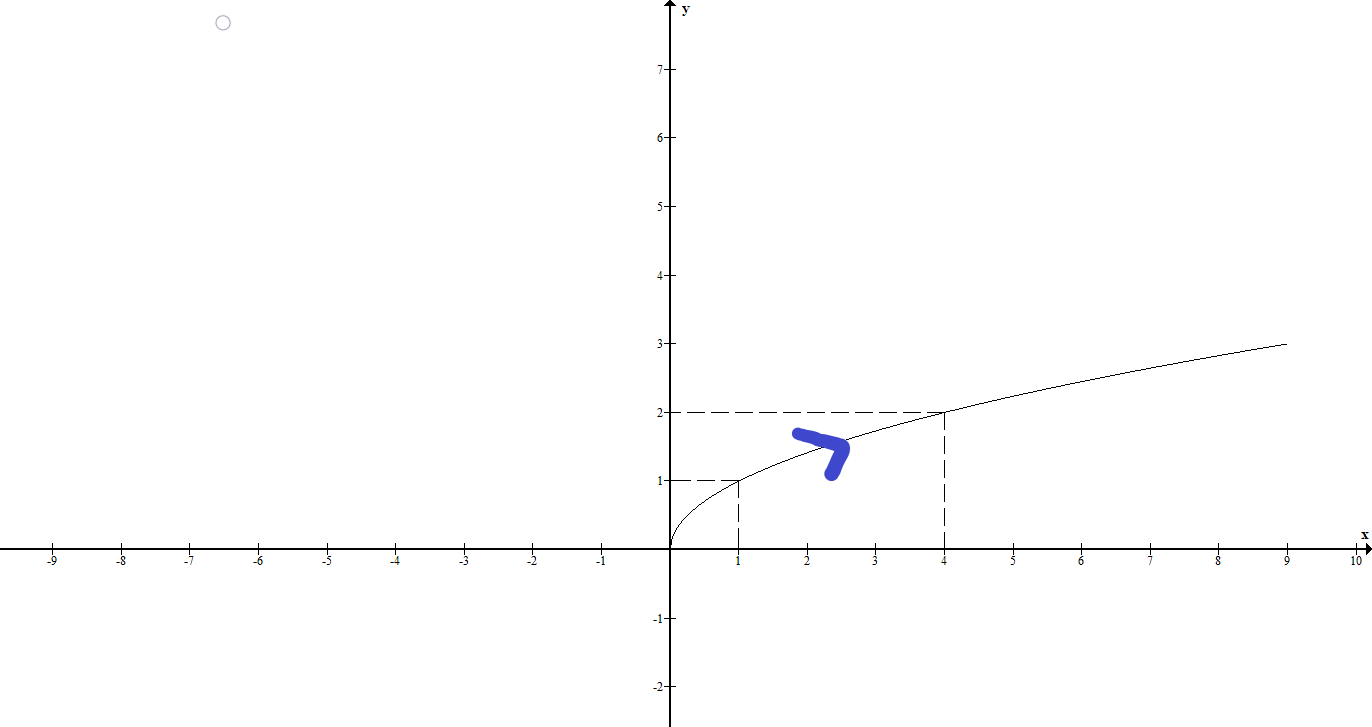
\includegraphics[scale=0.3]{c4_3}
\end{center}
Một tham số của \(C\) là
\[\left\{ \begin{gathered}
  x = t \hfill \\
  y = \sqrt t  \hfill \\ 
\end{gathered}  \right.,t \in \left[ {1,4} \right].\]
\[ \Rightarrow \frac{{dy}}{{dt}} = \frac{1}{{2\sqrt t }}.\]
\[ \Rightarrow I = \int\limits_1^4 {\left( {{t^2} \cdot t\sqrt t  - \sqrt t } \right)}  \cdot \frac{1}{{2\sqrt t }}dt\]
\[ \Rightarrow I = \frac{1}{2}\int\limits_1^4 {\left( {{t^3} - 1} \right)dt = \frac{1}{2}} \left. {\left( {\frac{{{t^4}}}{4} - t} \right)} \right|_{t = 1}^{t = 4} = \frac{{243}}{8}.\]
\textbf{Bài 3.}
\begin{mybox}
Tính tích phân đường loại \(2:\) \(I = \int_C {xydx + \left( {x - y} \right)dy} \) với \(C\) gồm các đoạn thẳng từ \(\left( {0,0} \right)\) đến \(\left( {2,0} \right)\) và từ \(\left( {2,0} \right)\) đến \(\left( {3,2} \right).\)
\end{mybox}
\begin{center}
	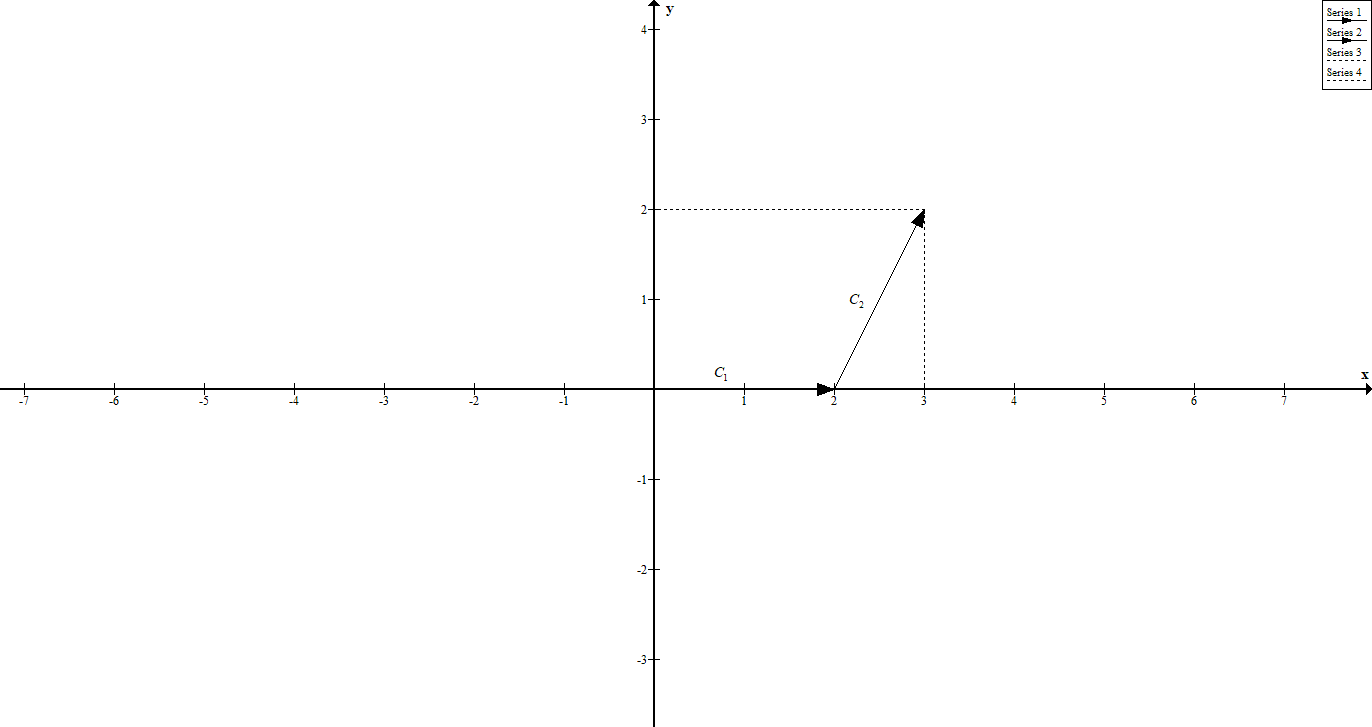
\includegraphics[scale=0.3]{c4_4}
\end{center}
Ta chia \(C\) thành 2 phần: \(C_1\) là đoạn thẳng nối từ \(\left( {0,0} \right)\) đến \(\left( {2,0} \right),\) \(C_2\) là đoạn thẳng nối từ \(\left( {2,0} \right)\) đến \(\left( {3,2} \right).\)
\[ \Rightarrow I = \int_C {xydx + \left( {x - y} \right)dy}  = \int_{{C_1} \cup {C_2}} {xydx + \left( {x - y} \right)dy} \]
\[ \Rightarrow I = \int_{{C_1}} {xydx + \left( {x - y} \right)dy}  + \int_{{C_2}} {xydx + \left( {x - y} \right)dy} .\]
Một tham số của \(C_1\) là
\[\left\{ \begin{gathered}
  x = t \hfill \\
  y = 0 \hfill \\ 
\end{gathered}  \right.,t \in \left[ {0,2} \right].\]
\[ \Rightarrow \left\{ \begin{gathered}
  \frac{{dx}}{{dt}} = 1 \hfill \\
  \frac{{dy}}{{dt}} = 0 \hfill \\ 
\end{gathered}  \right..\]
\[ \Rightarrow \int_{{C_1}} {xydx + \left( {x - y} \right)dy}  = \int\limits_0^2 {0dt}  = 0.\]
Phương trình đường thẳng  nối từ \(\left( {2,0} \right)\) đến \(\left( {3,2} \right)\) là \(y = 2x - 4.\)\\
\(\Rightarrow\) Một tham số của \(C_2\) là
\[\left\{ \begin{gathered}
  x = t \hfill \\
  y = 2t - 4 \hfill \\ 
\end{gathered}  \right.,t \in \left[ {2,3} \right].\]
\[ \Rightarrow \left\{ \begin{gathered}
  \frac{{dx}}{{dt}} = 1 \hfill \\
  \frac{{dy}}{{dt}} = 2 \hfill \\ 
\end{gathered}  \right..\]
\[ \Rightarrow \int_{{C_2}} {xydx + \left( {x - y} \right)dy}  = \int\limits_2^3 {t\left( {2t - 4} \right)dt + \left[ {t - \left( {2t - 4} \right)} \right]2dt} \]
\[ \Rightarrow \int_{{C_2}} {xydx + \left( {x - y} \right)dy}  = \int\limits_2^3 {\left( {2{t^2} - 6t + 8} \right)dt}  = \frac{{17}}{3}.\]
\[ \Rightarrow I = 0 + \frac{{17}}{3} = \frac{{17}}{3}.\]
\textbf{Bài 4.}
\begin{mybox}
Tính tích phân đường loại \(2:\) \(I = \int_C {\sin xdx + \cos ydy} \) với \(C\) gồm nửa trên của đường tròn \({x^2} + {y^2} = 1\) từ \(\left( {1,0} \right)\) đến \(\left( { - 1,0} \right)\) và đoạn thẳng từ \(\left( { - 1,0} \right)\) đến \(\left( { - 2,3} \right).\)
\end{mybox}
\begin{center}
	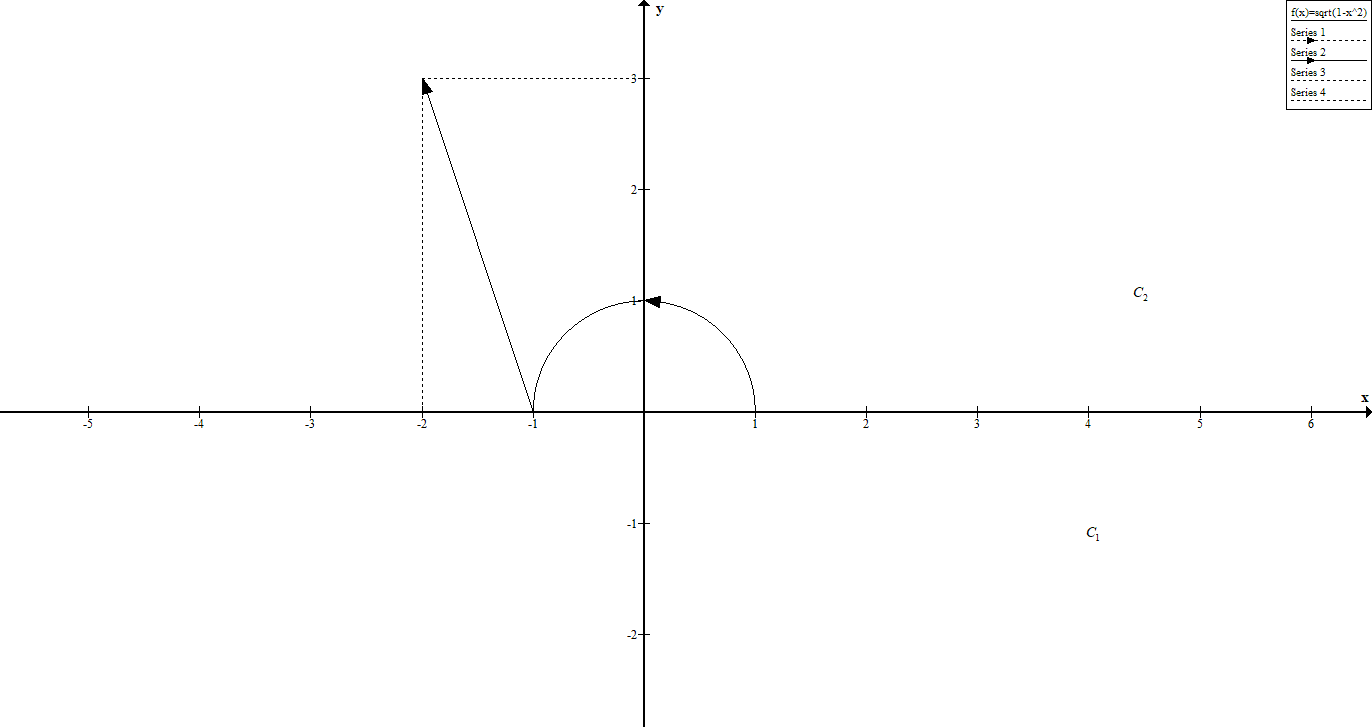
\includegraphics[scale=0.3]{c4_5}
\end{center}
Ta chia \(C\) thành \(2\) phần: \(C_1\) là nửa trên của đường tròn \({x^2} + {y^2} = 1\) từ \(\left( {1,0} \right)\) đến \(\left( { - 1,0} \right)\) và \(C_2\) là đoạn thẳng từ \(\left( { - 1,0} \right)\) đến \(\left( { - 2,3} \right).\)
\[ \Rightarrow I = \int_C {\sin xdx + \cos ydy}  = \int_{{C_1} \cup {C_2}} {\sin xdx + \cos ydy} \]
\[ \Rightarrow I = \int_{{C_1}} {\sin xdx + \cos ydy}  + \int_{{C_2}} {\sin xdx + \cos ydy} .\]
Một tham số của \(C_1\) là
\[\left\{ \begin{gathered}
  x = \cos t \hfill \\
  y = \sin t \hfill \\ 
\end{gathered}  \right.,t \in \left[ {0,\pi } \right].\]
\[ \Rightarrow \left\{ \begin{gathered}
  \frac{{dx}}{{dt}} =  - \sin t \hfill \\
  \frac{{dy}}{{dt}} = \cos t \hfill \\ 
\end{gathered}  \right..\]
\[ \Rightarrow {I_1} = \int_{{C_1}} {\sin xdx + \cos ydy}  = \int\limits_0^\pi  {\sin \left( {\cos t} \right)\left( { - \sin t} \right)} dt + \cos \left( {\sin t} \right)\cos tdt\]
\[ \Rightarrow {I_1} = \int\limits_0^\pi  {\sin \left( {\cos t} \right)\left( { - \sin t} \right)} dt + \int\limits_0^\pi  {\cos \left( {\sin t} \right)\cos tdt} \]
\[ \Rightarrow {I_1} = \left. { - \cos \left( {\cos t} \right)} \right|_{t = 0}^{t = \pi } + \left. {\sin \left( {\sin t} \right)} \right|_{t = 0}^{t = \pi } =  - \cos \left( { - 1} \right) + \cos \left( 1 \right) + \sin \left( 0 \right) - \sin \left( 0 \right) = 0.\]
Phương trình đường thẳng nối từ \(\left( { - 1,0} \right)\) đến \(\left( { - 2,3} \right)\) là \(y = -3x - 3.\)\\
\(\Rightarrow\) Một tham số của \(C_2\) là
\[\left\{ \begin{gathered}
  x =  - t \hfill \\
  y = 3t - 3 \hfill \\ 
\end{gathered}  \right.,t \in \left[ {1,2} \right].\]
\[ \Rightarrow \left\{ \begin{gathered}
  \frac{{dx}}{{dt}} =  - 1 \hfill \\
  \frac{{dy}}{{dt}} = 3 \hfill \\ 
\end{gathered}  \right..\]
\[ \Rightarrow {I_2} = \int_{{C_2}} {\sin xdx + \cos ydy}  = \int\limits_1^2 {\left[ {\sin \left( { - t} \right)\left( { - dt} \right) + \cos \left( {3t - 3} \right) \cdot 3dt} \right]} \]
\[ \Rightarrow {I_2} = \int\limits_1^2 {\left[ {\sin t + 3\cos \left( {3t - 3} \right)} \right]} dt = \left. {\left[ { - \cos t + \sin \left( {3t - 3} \right)} \right]} \right|_{t = 1}^{t = 2} = \cos \left( 1 \right) - \cos \left( 2 \right) + \sin \left( 3 \right).\]
\textbf{Bài 5.}
\begin{mybox}
Tính tích phân đường loại \(2:\) \(I = \int_C {{x^2}y\sqrt z dz} \) với \(C:x = {t^3},y = t,z = {t^2},\) \(0 \leqslant t \leqslant 1.\)
\end{mybox}
\[z = {t^2} \Rightarrow \frac{{dz}}{{dt}} = 2t.\]
\[ \Rightarrow I = \int\limits_0^1 {{t^6} \cdot t \cdot t \cdot 2tdt}  = 2\int\limits_0^1 {{t^9}} dt = \left. {\frac{{{t^{10}}}}{5}} \right|_{t = 0}^{t = 1} = \frac{1}{5}.\]
\textbf{Bài 9.}
\begin{mybox}
Tính tích phân \(I = \int_C {\overrightarrow{F}d\overrightarrow{r}}\) với \(\overrightarrow F \left( {x,y} \right) = xy\overrightarrow i  + 3{y^2}\overrightarrow j \) và \(C\) là vết của đường đi \(\overrightarrow{r}\) định bởi \(r\left( t \right) = 11{t^4}\overrightarrow i  + {t^3}\overrightarrow j ,\) \(0 \leqslant t \leqslant 1.\)
\end{mybox}
\[\overrightarrow F \left( {x,y} \right) = \left\langle {xy,3{y^2}} \right\rangle  = \left\langle {P\left( {x,y} \right),Q\left( {x,y} \right)} \right\rangle .\]
\[ \Rightarrow \left\{ \begin{gathered}
  P\left( {x,y} \right) = xy \hfill \\
  Q\left( {x,y} \right) = 3{y^2} \hfill \\ 
\end{gathered}  \right..\]
\[\overrightarrow r \left( t \right) = \left\langle {11{t^4},{t^3}} \right\rangle  = \left\langle {x\left( t \right),y\left( t \right)} \right\rangle .\]
\[ \Rightarrow \left\{ \begin{gathered}
  x\left( t \right) = 11{t^4} \hfill \\
  y\left( t \right) = {t^3} \hfill \\ 
\end{gathered}  \right..\]
\[ \Rightarrow \left\{ \begin{gathered}
  x\left( t \right) = 11{t^4} \hfill \\
  y\left( t \right) = {t^3} \hfill \\ 
\end{gathered}  \right..\]
\[ \Rightarrow I = \int_C {Pdx + Qdy} \]
\[ \Rightarrow I = \int\limits_0^1 {\left[ {P\left( {x\left( t \right),y\left( t \right)} \right) \cdot x'\left( t \right) + Q\left( {x\left( t \right),y\left( t \right)} \right) \cdot y'\left( t \right)} \right]} dt\]
\[ \Rightarrow I = \int\limits_0^1 {\left( {11{t^4} \cdot {t^3} \cdot 44{t^3} + 3 \cdot {{\left( {{t^3}} \right)}^2} \cdot 3{t^2}} \right)} dt\]
\[ \Rightarrow I = \int\limits_0^1 {\left( {484{t^{10}} + 9{t^8}} \right)} dt = \left. {\left( {44{t^{11}} + {t^9}} \right)} \right|_{t = 0}^{t = 1} = 45.\]
\textbf{Trang 78.}\\
\textbf{Bài 1.}
\begin{mybox}
Tính tích phân đường \(I = \oint_C {\left( {x - y} \right)dx + \left( {x + y} \right)dy} \) với \(C\) là đường tròn có tâm ở gốc tọa độ, bán kính \(2\) theo 2 cách:\\
a. Tính trực tiếp.\\
b. Dùng định lí Green.
\end{mybox}
\begin{center}
	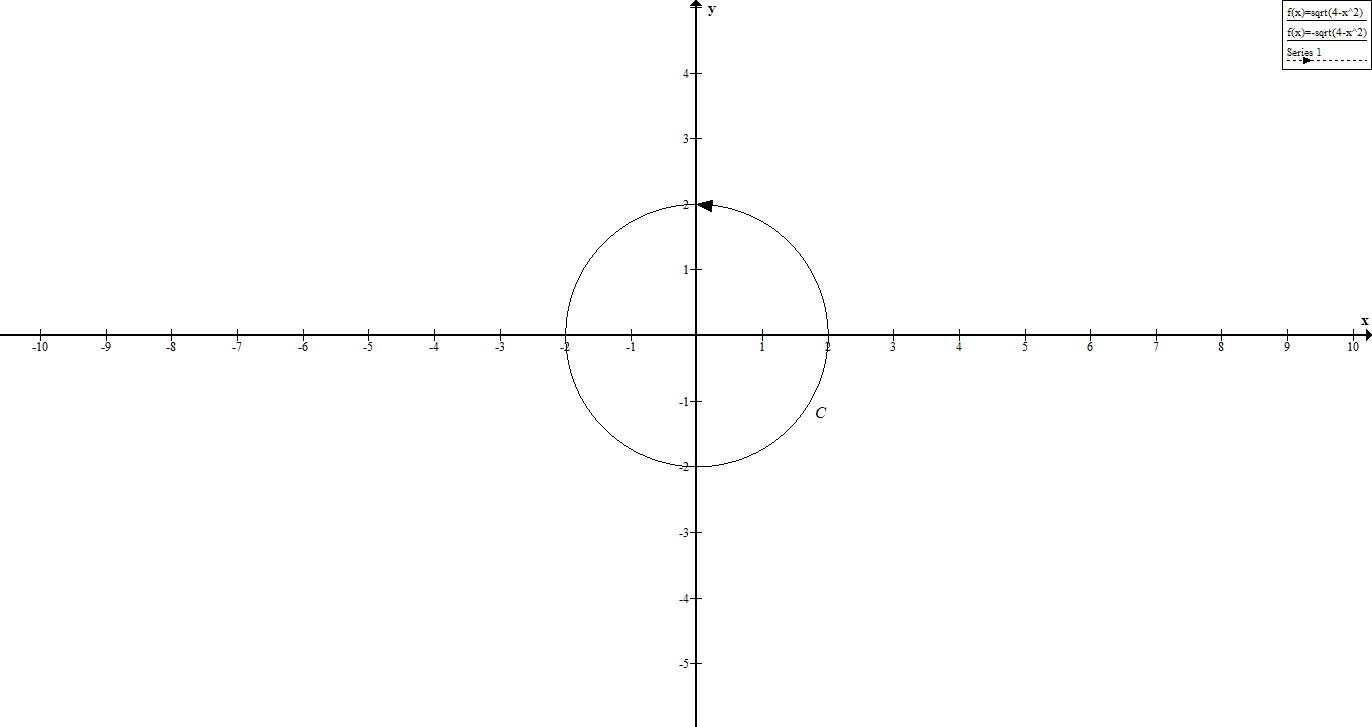
\includegraphics[scale=0.3]{c4_6}
\end{center}
\textbf{a. Tính trực tiếp.}\\
Một tham số của \(C\) là
\[\left\{ \begin{gathered}
  x = 2\cos t \hfill \\
  y = 2\sin t \hfill \\ 
\end{gathered}  \right.,t \in \left[ {0,2\pi } \right].\]
\[ \Rightarrow \left\{ \begin{gathered}
  \frac{{dx}}{{dt}} =  - 2\sin t \hfill \\
  \frac{{dy}}{{dt}} = 2\cos t \hfill \\ 
\end{gathered}  \right..\]
\[ \Rightarrow I = \int\limits_0^{2\pi } {\left( {2\cos t - 2\sin t} \right)\left( { - 2\sin t} \right)dt + \left( {2\cos  + 2\sin t} \right)2\cos tdt} \]
\[ \Rightarrow I = \int\limits_0^{2\pi } {4dt}  = \left. {4t} \right|_{t = 0}^{t = 2\pi } = 8\pi .\]
\textbf{b. Dùng định lí Green.}
\[D = \left\{ {\left. {\left( {r,\theta } \right)} \right|0 \leqslant r \leqslant 2,0 \leqslant \theta  \leqslant 2\pi } \right\}.\]
Đặt \(\left\{ \begin{gathered}
  P\left( {x,y} \right) = x - y \hfill \\
  Q\left( {x,y} \right) = x + y \hfill \\ 
\end{gathered}  \right. \Rightarrow \left\{ \begin{gathered}
  \frac{{\partial P}}{{\partial y}} =  - 1 \hfill \\
  \frac{{\partial Q}}{{\partial x}} = 1 \hfill \\ 
\end{gathered}  \right..\)
\[ \Rightarrow I = \int {\int_D {\left( {\frac{{\partial Q}}{{\partial x}} - \frac{{\partial P}}{{\partial y}}} \right)} } dA = \int\limits_0^{2\pi } {\int\limits_0^2 {2rdrd\theta } } \]
\[ \Rightarrow I = \int {\int_D {\left( {\frac{{\partial Q}}{{\partial x}} - \frac{{\partial P}}{{\partial y}}} \right)} } dA = \int\limits_0^{2\pi } {\int\limits_0^2 {2rdrd\theta } } \]
\textbf{Bài 2.}
\begin{mybox}
Tính tích phân đường \(I = \oint_C {xydx + {x^2}dy} \) với \(C\) là hình chữ nhật có các đỉnh \(\left( {0,0} \right),\left( {3,0} \right),\left( {3,1} \right),\left( {0,1} \right)\) theo 2 cách:\\
a. Tính trực tiếp.\\
b. Dùng định lí Green.
\end{mybox}
\begin{center}
	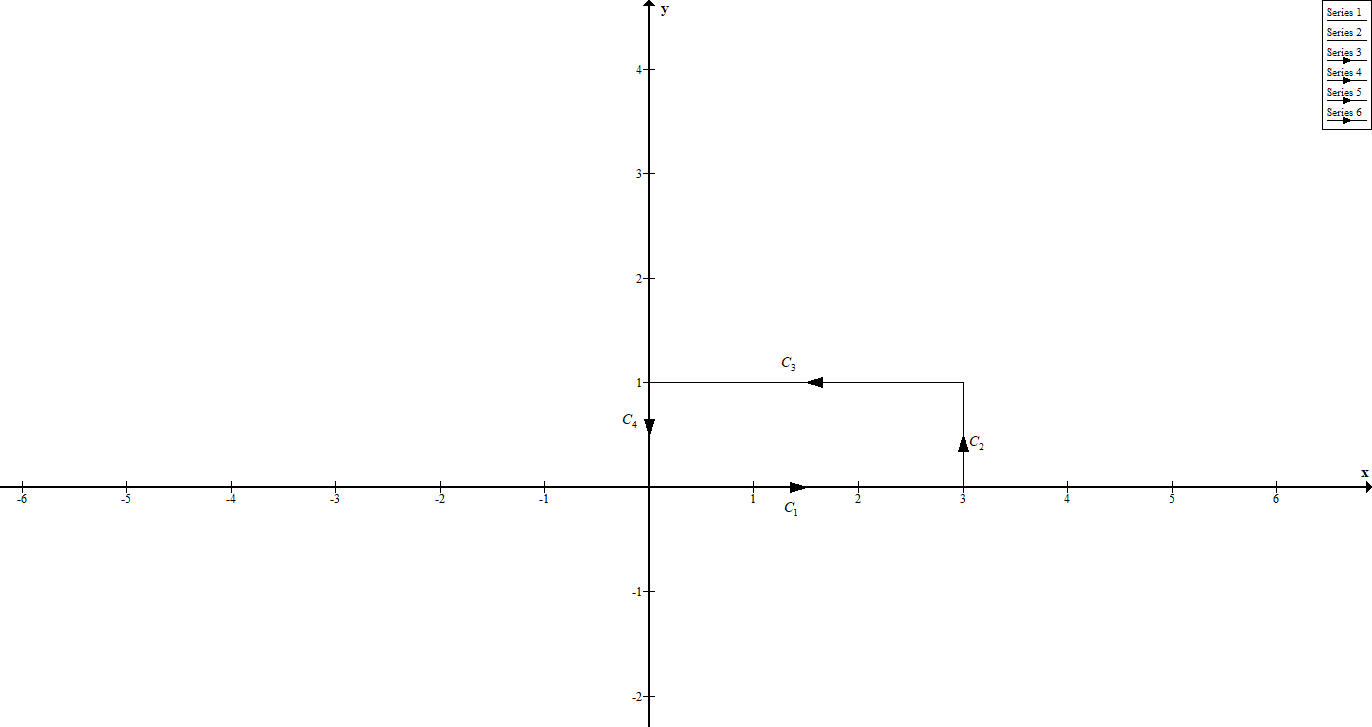
\includegraphics[scale=0.3]{c4_7}
\end{center}
\textbf{a. Tính trực tiếp.}\\
Ta chia \(C\) thành \(4\) đường cong \(C_1, C_2, C_3, C_4.\)
\begin{itemize}
\item \(C_1\) là đoạn nối từ \(\left( {0,0} \right)\) đến \(\left( {3,0} \right).\) Một tham số của \(C_1\) là
\[\left\{ \begin{gathered}
  x = t \hfill \\
  y = 0 \hfill \\ 
\end{gathered}  \right.,t \in \left[ {0,3} \right].\]
\[ \Rightarrow \left\{ \begin{gathered}
  \frac{{dx}}{{dt}} = 1 \hfill \\
  \frac{{dy}}{{dt}} = 0 \hfill \\ 
\end{gathered}  \right..\]
\item \(C_2\) là đoạn nối từ \(\left( {3,0} \right)\) đến \(\left( {3,1} \right).\) Một tham số của \(C_2\) là
\[\left\{ \begin{gathered}
  x = 3 \hfill \\
  y = t \hfill \\ 
\end{gathered}  \right.,t \in \left[ {0,1} \right].\]
\[ \Rightarrow \left\{ \begin{gathered}
  \frac{{dx}}{{dt}} = 0 \hfill \\
  \frac{{dy}}{{dt}} = 1 \hfill \\ 
\end{gathered}  \right..\]
\item \(C_3\) là đoạn nối từ \(\left( {3,1} \right)\) đến \(\left( {0,1} \right).\) Một tham số của \(C_3\) là
\[\left\{ \begin{gathered}
  x =  - t \hfill \\
  y = 1 \hfill \\ 
\end{gathered}  \right.,t \in \left[ { - 3,0} \right].\]
\[ \Rightarrow \left\{ \begin{gathered}
  \frac{{dx}}{{dt}} =  - 1 \hfill \\
  \frac{{dy}}{{dt}} = 0 \hfill \\ 
\end{gathered}  \right..\]
\item \(C_4\) là đoạn nối từ \(\left( {0,1} \right)\) đến \(\left( {0,0} \right).\) Một tham số của \(C_4\) là
\[\left\{ \begin{gathered}
  x = 0 \hfill \\
  y =  - t \hfill \\ 
\end{gathered}  \right.,t \in \left[ { - 1,0} \right].\]
\[ \Rightarrow \left\{ \begin{gathered}
  \frac{{dx}}{{dt}} = 0 \hfill \\
  \frac{{dy}}{{dt}} =  - 1 \hfill \\ 
\end{gathered}  \right..\]
\end{itemize}
\[I = \oint_C {xydx + {x^2}dy = \oint_{{C_1} \cup {C_2} \cup {C_3} \cup {C_4}} {xydx + {x^2}dy} } \]
\[ \Rightarrow I = \int_{{C_1}} {xydx + {x^2}dy}  + \int_{{C_2}} {xydx + {x^2}dy}  + \int_{{C_3}} {xydx + {x^2}dy}  + \int_{{C_4}} {xydx + {x^2}dy}. \]
\[\int_{{C_1}} {xydx + {x^2}dy}  = \int\limits_0^3 0 dt = 0.\]
\[\int_{{C_2}} {xydx + {x^2}dy}  = \int\limits_0^1 {3t \cdot 0 + 9dt}  = \int\limits_0^1 {9dt}  = 9.\]
\[\int_{{C_3}} {xydx + {x^2}dy}  = \int\limits_{ - 3}^0 {\left( { - t} \right)\left( { - dt} \right) + {x^2} \cdot 0}  = \int\limits_{ - 3}^0 {tdt = \left. {\frac{{{t^2}}}{2}} \right|} _{t =  - 3}^{t = 0} =  - \frac{9}{2}.\]
\[\int_{{C_4}} {xydx + {x^2}dy}  = \int\limits_{ - 1}^0 {0dt}  = 0.\]
\[ \Rightarrow I = 0 + 9 - \frac{9}{2} + 0 = \frac{9}{2}.\]
\textbf{b. Dùng định lí Green.}
\[D = \left\{ {\left. {\left( {x,y} \right)} \right|0 \leqslant x \leqslant 3,0 \leqslant y \leqslant 1} \right\}.\]
Đặt \(\left\{ \begin{gathered}
  P\left( {x,y} \right) = xy \hfill \\
  Q\left( {x,y} \right) = {x^2} \hfill \\ 
\end{gathered}  \right. \Rightarrow \left\{ \begin{gathered}
  \frac{{\partial P}}{{\partial y}} = x \hfill \\
  \frac{{\partial Q}}{{\partial x}} = 2x \hfill \\ 
\end{gathered}  \right..\)
\[I = \int {\int_D {\left( {\frac{{\partial Q}}{{\partial x}} - \frac{{\partial P}}{{\partial y}}} \right)} } dA = \int\limits_0^3 {\int\limits_0^1 {\left( {2x - x} \right)dydx} } \]
\[ \Rightarrow I = \int\limits_0^3 {\int\limits_0^1 {xdydx} }  = \int\limits_0^3 {\left( {\left. {xy} \right|_{y = 0}^{y = 1}} \right)} dx = \int\limits_0^3 {xdx}  = \left. {\frac{{{x^2}}}{2}} \right|_{x = 0}^{x = 3} = \frac{9}{2}.\]
\textbf{Bài 3.}
\begin{mybox}
Tính tích phân đường \(I = \oint_C {xydx + {x^2}{y^3}dy} \) với \(C\) là hình tam giác có các đỉnh là \(\left( {0,0} \right),\left( {1,0} \right),\left( {1,2} \right)\) theo 2 cách:\\
a. Tính trực tiếp.\\
b. Dùng định lí Green.
\end{mybox}
\begin{center}
	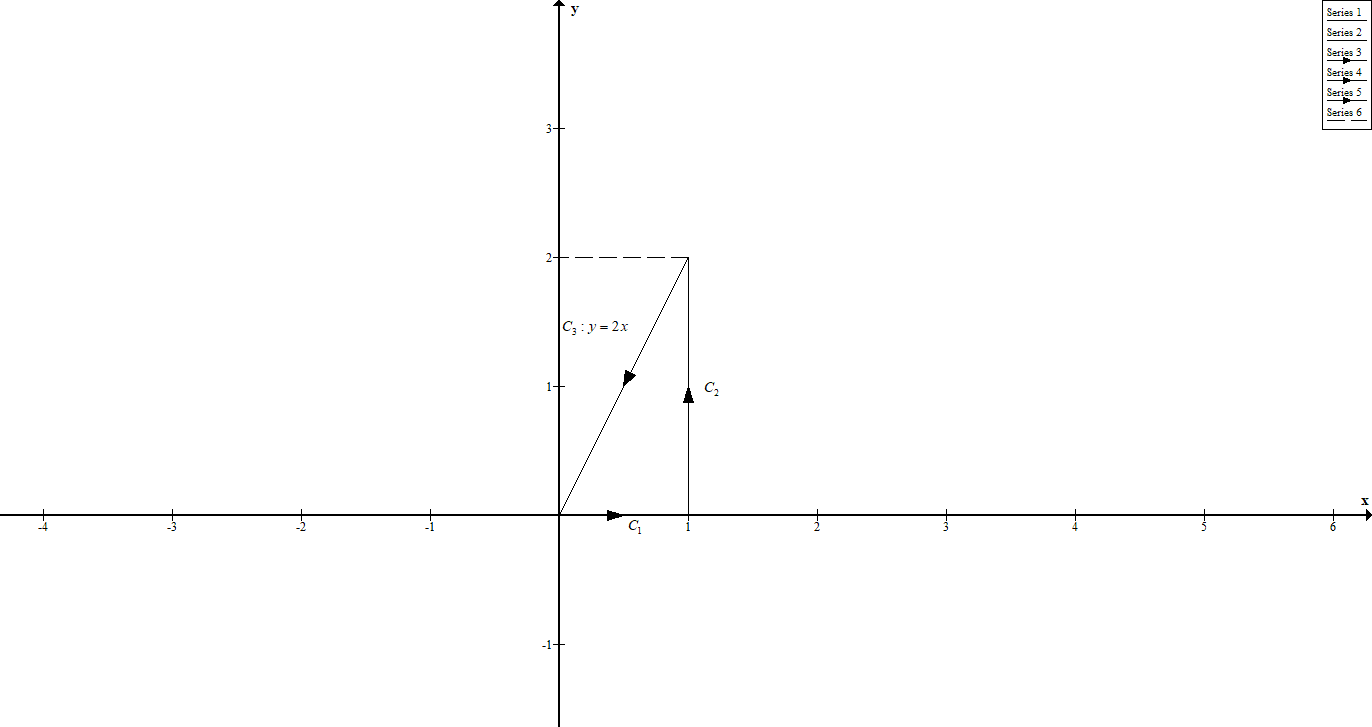
\includegraphics[scale=0.3]{c4_8}
\end{center}
\textbf{a. Tính trực tiếp.}\\
Ta chia \(C\) thành \(3\) đường cong: \(C_1, C_2, C_3.\)
\begin{itemize}
	\item \(C_1\) là đoạn nối từ \(\left( {0,0} \right)\) đến \(\left( {1,0} \right).\) Một tham số của \(C_1\) là
\[\left\{ \begin{gathered}
  x = t \hfill \\
  y = 0 \hfill \\ 
\end{gathered}  \right.,t \in \left[ {0,1} \right].\]
\[ \Rightarrow \left\{ \begin{gathered}
  \frac{{dx}}{{dt}} = 1 \hfill \\
  \frac{{dy}}{{dt}} = 0 \hfill \\ 
\end{gathered}  \right..\]
\item \(C_2\) là đoạn nối từ \(\left( {1,0} \right)\) đến \(\left( {1,2} \right).\) Một tham số của \(C_2\) là
\[\left\{ \begin{gathered}
  x = 1 \hfill \\
  y = t \hfill \\ 
\end{gathered}  \right.,t \in \left[ {0,2} \right].\]
\[ \Rightarrow \left\{ \begin{gathered}
  \frac{{dx}}{{dt}} = 0 \hfill \\
  \frac{{dy}}{{dt}} = 1 \hfill \\ 
\end{gathered}  \right..\]
\item \(C_3\) là đoạn nối từ \(\left( {1,2} \right)\) đến \(\left( {0,0} \right).\) Một tham số của \(C_3\) là
\[\left\{ \begin{gathered}
  x = t \hfill \\
  y =  - 2t \hfill \\ 
\end{gathered}  \right.,t \in \left[ { - 1,0} \right].\]
\[ \Rightarrow \left\{ \begin{gathered}
  \frac{{dx}}{{dt}} = 1 \hfill \\
  \frac{{dy}}{{dt}} =  - 2 \hfill \\ 
\end{gathered}  \right..\]
\end{itemize}
\[I = \oint_C {xydx + {x^2}{y^3}dy}  = \oint_{{C_1} \cup {C_2} \cup {C_3}} {xydx + {x^2}{y^3}dy} \]
\[ \Rightarrow I = \int_{{C_1}} {xydx + {x^2}{y^3}dy}  + \int_{{C_2}} {xydx + {x^2}{y^3}dy}  + \int_{{C_3}} {xydx + {x^2}{y^3}dy} .\]
\[\int_{{C_1}} {xydx + {x^2}{y^3}dy}  = \int\limits_0^1 {0dt}  = 0.\]
\[\int_{{C_2}} {xydx + {x^2}{y^3}dy}  = \int\limits_0^2 {\left( {t \cdot 0 + {t^3}} \right)} dt = \int\limits_0^2 {{t^3}} dt = \left. {\frac{{{t^4}}}{4}} \right|_{t = 0}^{t = 2} = 4.\]
\[\int_{{C_3}} {xydx + {x^2}{y^3}dy}  = \int\limits_{ - 1}^0 {t\left( { - 2t} \right)} dt + {t^2}{\left( { - 2t} \right)^3}\left( { - 2dt} \right) = \int\limits_{ - 1}^0 {\left( { - 2{t^2} + 16{t^5}} \right)dt = \left. {\left( { - \frac{2}{3}{t^3} + \frac{8}{3}{t^6}} \right)} \right|} _{t =  - 1}^{t = 0} =  - \frac{{10}}{3}.\]
\[ \Rightarrow I = 0 + 4 - \frac{{10}}{3} = \frac{2}{3}.\]
\textbf{b. Dùng định lí Green.}
\[D = \left\{ {\left. {\left( {x,y} \right)} \right|0 \leqslant x \leqslant 1,0 \leqslant y \leqslant 2x} \right\}.\]
Đặt \(\left\{ \begin{gathered}
  Px,y = xy \hfill \\
  Qx,y = {x^2}{y^3} \hfill \\ 
\end{gathered}  \right. \Rightarrow \left\{ \begin{gathered}
  \frac{{\partial P}}{{\partial y}} = x \hfill \\
  \frac{{\partial Q}}{{\partial x}} = 2x{y^3} \hfill \\ 
\end{gathered}  \right..\)
\[I = \int {\int_D {\left( {\frac{{\partial Q}}{{\partial x}} - \frac{{\partial P}}{{\partial y}}} \right)} } dA = \int\limits_0^1 {\int\limits_0^{2x} {\left( {2x{y^3} - x} \right)} dydx} \]
\[ \Rightarrow I = \int\limits_0^1 {\left. {\left( {\frac{{x{y^4}}}{2} - xy} \right)} \right|} _{y = 0}^{y = 2x}dx = \int\limits_0^1 {\left( {8{x^5} - 2{x^2}} \right)} dx\]
\[ \Rightarrow I = \left. {\left( {\frac{4}{3}{x^6} - \frac{2}{3}{x^3}} \right)} \right|_{x = 0}^{x = 1} = \frac{2}{3}.\]
\textbf{Trang 79.}\\
\textbf{Bài 4.}
\begin{mybox}
Tính tích phân đường \(I = \oint_C {xdx + ydy} \) với \(C\) là đoạn thẳng từ \(\left( {0,1} \right)\) đến \(\left( {0,0} \right),\) từ \(\left( {0,0} \right)\) đến \(\left( {1,0} \right)\) và đoạn parabola \(\left( {1,0} \right)\) từ \(\left( {1,0} \right)\) đến \(\left( {0,1} \right)\) theo 2 cách:\\
a. Tính trực tiếp.\\
b. Dùng định lí Green.
\end{mybox}
\begin{center}
	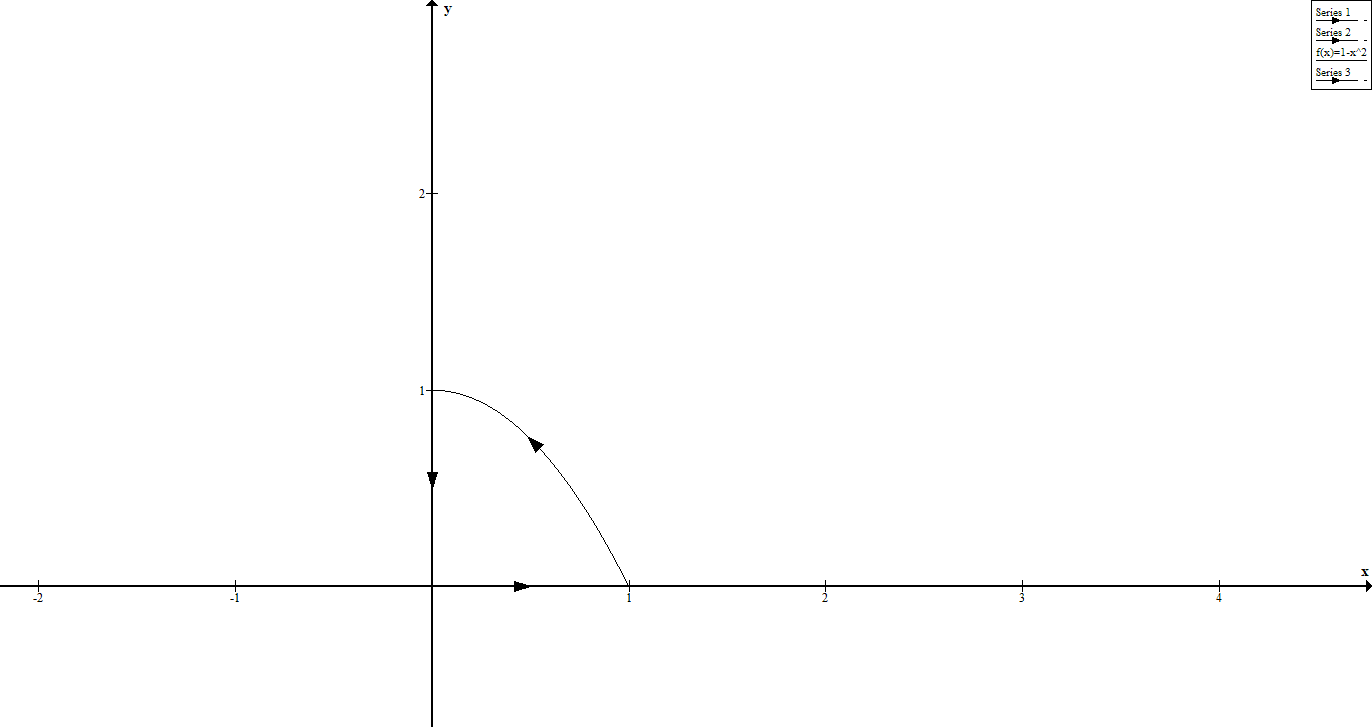
\includegraphics[scale=0.3]{c4_9}
\end{center}
a. \textbf{Tính trực tiếp.}\\
Ta chia \(C\) thành \(3\) đường cong: \(C_1, C_2, C_3.\)
\begin{itemize}
	\item \(C_1\) là đoạn thẳng nối từ từ \(\left( {0,1} \right)\) đến \(\left( {0,0} \right).\) Một tham số của \(C_1\) là
	\[\left\{ \begin{gathered}
  x = 0 \hfill \\
  y =  - t \hfill \\ 
\end{gathered}  \right.,t \in \left[ { - 1,0} \right].\]
\[ \Rightarrow \left\{ \begin{gathered}
  \frac{{dx}}{{dt}} = 0 \hfill \\
  \frac{{dy}}{{dt}} =  - 1 \hfill \\ 
\end{gathered}  \right..\]
\item \(C_2\) là đoạn thẳng nối từ \(\left( {0,0} \right)\) đến \(\left( {1,0} \right).\) Một tham số của \(C_2\) là 
\[\left\{ \begin{gathered}
  x = t \hfill \\
  y = 0 \hfill \\ 
\end{gathered}  \right.,t \in \left[ {0,1} \right].\]
\[ \Rightarrow \left\{ \begin{gathered}
  \frac{{dx}}{{dt}} = 1 \hfill \\
  \frac{{dy}}{{dt}} = 0 \hfill \\ 
\end{gathered}  \right..\]
\item \(C_3\) là đoạn parabola \(\left( {1,0} \right)\) từ \(\left( {1,0} \right)\) đến \(\left( {0,1} \right).\) Một tham số của \(C_3\) là
\[\left\{ \begin{gathered}
  x =  - t \hfill \\
  y = 1 - {t^2} \hfill \\ 
\end{gathered}  \right.,t \in \left[ { - 1,0} \right].\]
\[ \Rightarrow \left\{ \begin{gathered}
  \frac{{dx}}{{dt}} =  - 1 \hfill \\
  \frac{{dy}}{{dt}} =  - 2t \hfill \\ 
\end{gathered}  \right..\]
\end{itemize}
\[I = \oint_C x dx + ydy = \oint_{{C_1} \cup {C_2} \cup {C_3}} x dx + ydy\]
\[ \Rightarrow I = \int_{{C_1}} {xdx + ydy}  + \int_{{C_2}} {xdx + ydy}  + \int_{{C_3}} {xdx + ydy} .\]
\[\int_{{C_1}} {xdx + ydy}  = \int\limits_{ - 1}^0 {0 + \left( { - t} \right)\left( { - dt} \right)}  = \int\limits_{ - 1}^0 {tdt}  =  - \frac{1}{2}.\]
\[\int_{{C_2}} {xdx + ydy}  = \int\limits_0^1 {tdt}  = \frac{1}{2}.\]
\[\int_{{C_3}} {xdx + ydy}  = \int\limits_{ - 1}^0 {\left( { - t} \right)\left( { - dt} \right) + \left( {1 - {t^2}} \right)\left( { - 2tdt} \right)}  = \int\limits_{ - 1}^0 {\left( {t - 2t + 2{t^3}} \right)dt}  = 0.\]
\[ \Rightarrow I =  - \frac{1}{2} + \frac{1}{2} + 0 = 0.\]
\textbf{b. Dùng định lí Green.}
\[D = \left\{ {\left. {\left( {x,y} \right)} \right|0 \leqslant x \leqslant 1,0 \leqslant y \leqslant 1 - {x^2}} \right\}.\]
Đặt \(\left\{ \begin{gathered}
  P\left( {x,y} \right) = x \hfill \\
  Q\left( {x,y} \right) = y \hfill \\ 
\end{gathered}  \right. \Rightarrow \left\{ \begin{gathered}
  \frac{{\partial P}}{{\partial y}} = 0 \hfill \\
  \frac{{\partial Q}}{{\partial x}} = 0 \hfill \\ 
\end{gathered}  \right..\)
\[I = \int {\int_D {\left( {\frac{{\partial Q}}{{\partial x}} - \frac{{\partial P}}{{\partial y}}} \right)} } dA = \int\limits_0^1 {\int\limits_0^{1 - {x^2}} {0dydx}  = \int\limits_0^1 {0dx}  = 0.} \]
\textbf{Bài 9.}
\begin{mybox}
Dùng định lí Green để tính tích phân \(I = \oint_C {{y^3}dx - {x^3}dy} \) dọc theo đường cong kín \(C\) với \(C\) là đường tròn \({x^2} + {y^2} = 4.\)
\end{mybox}
\begin{center}
	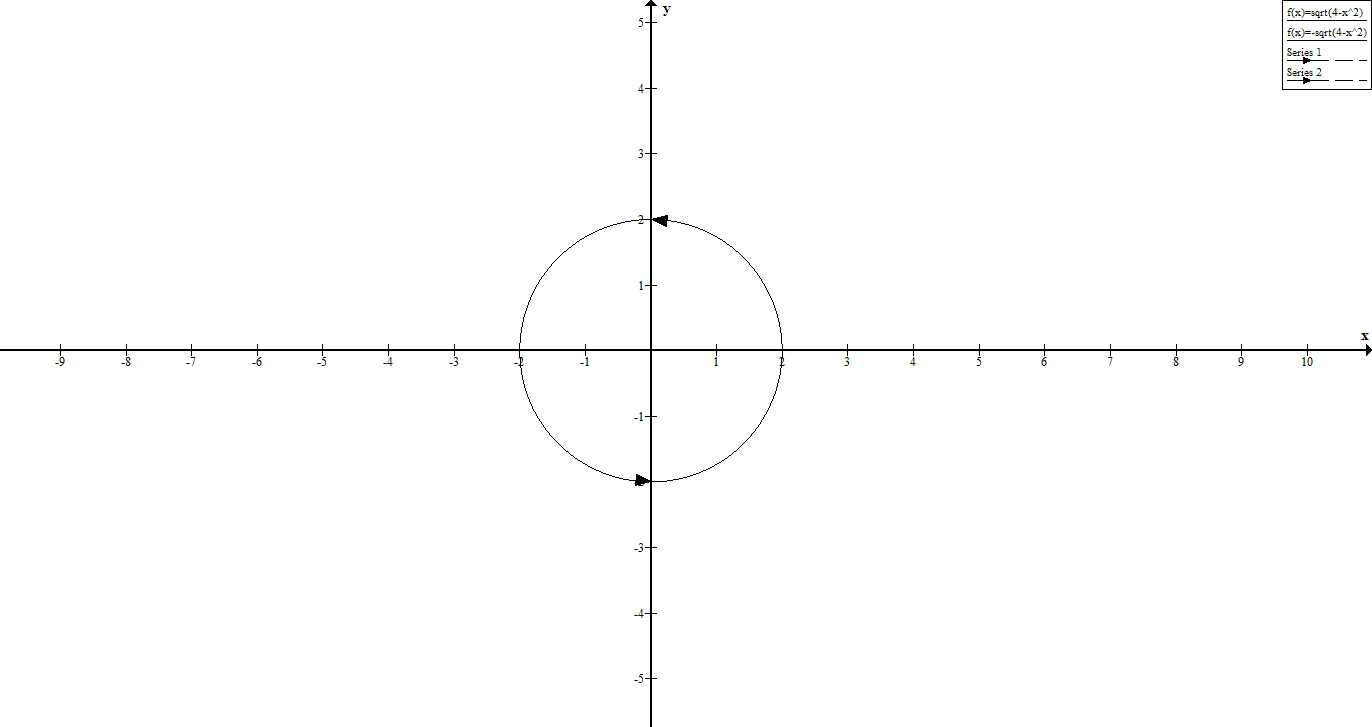
\includegraphics[scale=0.3]{c4_10}
\end{center}
\[D = \left\{ {\left. {\left( {r,\theta } \right)} \right|0 \leqslant r \leqslant 2,0 \leqslant \theta  \leqslant 2\pi } \right\}.\]
Đặt \(\left\{ \begin{gathered}
  P\left( {x,y} \right) = {y^3} \hfill \\
  Q\left( {x,y} \right) =  - {x^3} \hfill \\ 
\end{gathered}  \right. \Rightarrow \left\{ \begin{gathered}
  \frac{{\partial P}}{{\partial y}} = 3{y^2} \hfill \\
  \frac{{\partial Q}}{{\partial x}} =  - 3{x^2} \hfill \\ 
\end{gathered}  \right..\)
\[I = \int {\int_D {\left( {\frac{{\partial Q}}{{\partial x}} - \frac{{\partial P}}{{\partial y}}} \right)} } dA = \int\limits_0^{2\pi } {\int\limits_0^2 {\left( { - 3{r^2}{{\cos }^2}\theta  - 3{r^2}{{\sin }^2}\theta } \right)rdrd\theta } } \]
\[ \Rightarrow I = \int\limits_0^{2\pi } {\int\limits_0^2 { - 3{r^3}drd\theta }  = \int\limits_0^{2\pi } {\left( {\left. { - \frac{3}{4}{r^4}} \right|_{r = 0}^{r = 2}} \right)d\theta }  = \int\limits_0^{2\pi } {\left( { - 12} \right)d\theta } } \]
\[ \Rightarrow I = \left. {\left( { - 12\theta } \right)} \right|_{\theta  = 0}^{\theta  = 2\pi } =  - 24\pi .\]
\textbf{Trang 82.}\\
\textbf{Bài 5.}
\begin{mybox}
Xác định xem trường \(2\) chiều \(\overrightarrow{F}\) định bởi \(\overrightarrow F \left( {x,y} \right) = \left( {2x - 3y} \right)\overrightarrow i  + \left( { - 3x + 4y - 8} \right)\overrightarrow j \) có phải là trường bảo toàn không? Nếu có, tìm hàm thế \(f\) của trường này.
\end{mybox}
\[\overrightarrow F \left( {x,y} \right) = \left\langle {2x - 3y, - 3x + 4y - 8} \right\rangle .\]
\[\frac{\partial }{{\partial y}}\left( {2x - 3y} \right) =  - 3.\]
\[\frac{\partial }{{\partial x}}\left( { - 3x + 4y - 8} \right) =  - 3.\]
\[ \Rightarrow \frac{\partial }{{\partial y}}\left( {2x - 3y} \right) = \frac{\partial }{{\partial x}}\left( { - 3x + 4y - 8} \right).\]
\( \Rightarrow \overrightarrow F \) là trường bảo toàn trên \(\mathbb{R} ^2.\)
\[\int {\left( {2x - 3y} \right)dx}  = {x^2} - 3xy + C\left( y \right).\]
\[\frac{\partial }{{\partial y}}\left( {{x^2} - 3xy + C\left( y \right)} \right) =  - 3x + C'\left( y \right).\]
\[ \Rightarrow C'\left( y \right) = 4y - 8.\]
Ta chọn \(C\left( y \right) = 2{y^2} - 8y.\)\\
Vậy \(f\left( {x,y} \right) = {x^2} - 3xy + 4y - 8\) là một hàm thế của trường \(\overrightarrow{F}.\)\\
\textbf{Bài 6.}
\begin{mybox}
Xác định xem trường \(2\) chiều \(\overrightarrow{F}\) định bởi \(\overrightarrow F \left( {x,y} \right) = {e^x}\cos y\overrightarrow i  + {e^x}\sin y\overrightarrow j \) có phải là trường bảo toàn không? Nếu có, tìm hàm thế \(f\) của trường này.
\end{mybox}
\[\overrightarrow F \left( {x,y} \right) = \left\langle {{e^x}\cos y,{e^x}\sin y} \right\rangle .\]
\[\frac{\partial }{{\partial y}}\left( {{e^x}\cos y} \right) =  - {e^x}\sin y.\]
\[\frac{\partial }{{\partial x}}\left( {{e^x}\sin y} \right) = {e^x}\sin y.\]
\[ \Rightarrow \frac{\partial }{{\partial y}}\left( {{e^x}\cos y} \right) \ne \frac{\partial }{{\partial x}}\left( {{e^x}\sin y} \right).\]
\( \Rightarrow \overrightarrow F \) không là trường bảo toàn trên \(\mathbb{R}^2.\)\\
\textbf{Bài 13.}
\begin{mybox}
Chứng minh trường \(\overrightarrow{F}\) định bởi \(\overrightarrow{F} \left( {x,y} \right) = {x^2}\overrightarrow i  + {y^2}\overrightarrow j \) là trường bảo toàn, sau đó dùng hàm thế của \(\overrightarrow{F}\) để tính \(I = \int_C {\overrightarrow {F \cdot } d\overrightarrow r } \) với \(C\) là đoạn parabola \(y = 2{x^2}\) nối từ \(\left( { - 1,2} \right)\) đến \(\left( {2,8} \right).\)
\end{mybox}
\[\overrightarrow F \left( {x,y} \right) = \left\langle {{x^2},{y^2}} \right\rangle .\]
\[\frac{\partial }{{\partial y}}\left( {{x^2}} \right) = 0.\]
\[\frac{\partial }{{\partial x}}\left( {{y^2}} \right) = 0.\]
\[ \Rightarrow \frac{\partial }{{\partial y}}\left( {{x^2}} \right) = \frac{\partial }{{\partial x}}\left( {{y^2}} \right).\]
\( \Rightarrow \overrightarrow F \) là trường bảo toàn trên \(\mathbb{R}^2.\)
\[\int {{x^2}dx}  = \frac{1}{3}{x^3} + C\left( y \right).\]
\[\frac{\partial }{{\partial y}}\left( {\frac{1}{3}{x^3} + C\left( y \right)} \right) = C'\left( y \right).\]
\[ \Rightarrow C'\left( y \right) = {y^2}.\]
Ta chọn \(C\left( y \right) = \frac{1}{3}{y^3}.\)\\
\( \Rightarrow f\left( {x,y} \right) = \frac{1}{3}{x^3} + \frac{1}{3}{y^3}\) là một hàm thế của trường \(\overrightarrow{F}.\)
\[ \Rightarrow I = \int_C {\overrightarrow {F \cdot } d\overrightarrow r }  = f\left( {2,8} \right) - f\left( { - 1,2} \right) = \frac{{520}}{3} - \frac{7}{3} = 171.\]
\textbf{Bài 14.}
\begin{mybox}
Chứng minh trường \(\overrightarrow{F}\) định bởi \(\overrightarrow F \left( {x,y} \right) = x{y^2}\overrightarrow i  + {x^2}y\overrightarrow j \) là trường bảo toàn, sau đó dùng hàm thế của \(\overrightarrow{F}\) để tính \(I = \int_C {\overrightarrow F  \cdot d\overrightarrow r } \) với \(C:\overrightarrow r \left( t \right) = \left\langle {t + \sin \frac{1}{2}\pi t,t + \frac{1}{2}\cos \pi t} \right\rangle ,\) \(0 \leqslant t \leqslant 1.\)
\end{mybox}
\[\overrightarrow{F}\left( {x,y} \right) = \left\langle {x{y^2},{x^2}y} \right\rangle .\]
\[\frac{\partial }{{\partial y}}\left( {x{y^2}} \right) = 2xy.\]
\[\frac{\partial }{{\partial x}}\left( {{x^2}y} \right) = 2xy.\]
\[ \Rightarrow \frac{\partial }{{\partial y}}\left( {x{y^2}} \right) = \frac{\partial }{{\partial x}}\left( {{x^2}y} \right).\]
\( \Rightarrow \overrightarrow F \) là trường bảo toàn trên \(\mathbb{R}^2.\)
\[\int {x{y^2}dx}  = \frac{1}{2}{x^2}{y^2} + C\left( y \right).\]
\[\frac{\partial }{{\partial y}}\left( {\frac{1}{2}{x^2}{y^2} + C\left( y \right)} \right) = {x^2}y + C'\left( y \right).\]
\[ \Rightarrow C'\left( y \right) = 0.\]
Ta chọn \(C\left( y \right) = 0.\)\\
\( \Rightarrow f\left( {x,y} \right) = \frac{1}{2}{x^2}{y^2}\) là một hàm thế của trường \(\overrightarrow{F}.\)\\
Điểm đầu của \(C\) là \(\overrightarrow r \left( 0 \right) = \left( {0,\frac{1}{2}} \right),\) điểm cuối của \(C\) là  \(\overrightarrow r \left( 1 \right) = \left( {2,\frac{1}{2}} \right).\)
\[ \Rightarrow I = \int_C {\overrightarrow F  \cdot d\overrightarrow r }  = f\left( {2,\frac{1}{2}} \right) - f\left( {0,\frac{1}{2}} \right) = \frac{1}{2}.\]
\textbf{Bài 17.}
\begin{mybox}
Chứng minh rằng tích phân \(I = \int_C {\left( {1 - y{e^{ - x}}} \right)dx + {e^{ - x}}dy}, \) với \(C\) là bất kì đường đi nào nối từ \(\left( {0,1} \right)\) đến \(\left( {1,2} \right),\) độc lập với đường đi và tính tích phân đó.
\end{mybox}
Xét trường \(\overrightarrow{F}\) định bởi
\[\overrightarrow F \left( {x,y} \right) = \left\langle {1 - y{e^{ - x}},{e^{ - x}}} \right\rangle .\]
\[\frac{\partial }{{\partial y}}\left( {1 - y{e^{ - x}}} \right) =  - {e^{ - x}}.\]
\[\frac{\partial }{{\partial x}}\left( {{e^{ - x}}} \right) =  - {e^{ - x}}.\]
\[ \Rightarrow \frac{\partial }{{\partial y}}\left( {1 - y{e^{ - x}}} \right) = \frac{\partial }{{\partial x}}\left( {{e^{ - x}}} \right).\]
\( \Rightarrow \overrightarrow F \) là trường bảo toàn trên \(\mathbb{R}^2.\)\\
\( \Rightarrow \) Tích phân \(I\) độc lập với đường đi.
\[\int {\left( {1 - y{e^{ - x}}} \right)dx}  = x + y{e^{ - x}} + C\left( y \right).\]
\[\frac{\partial }{{\partial y}}\left( {x + y{e^{ - x}}} \right) = {e^{ - x}} + C'\left( y \right).\]
\[ \Rightarrow C'\left( y \right) = 0.\]
Ta chọn \(C\left( y \right) = 0.\)\\
\( \Rightarrow f\left( {x,y} \right) = x + y{e^{ - x}}\) là một hàm thế của trường \(\overrightarrow{F}.\)
\[ \Rightarrow I = f\left( {1,2} \right) - f\left( {0,1} \right) = 1 + \frac{2}{e} - 1 = \frac{2}{e}.\]
\end{document}